\chapter{Hamilton-Jacobi Theory}
\label{hj}

The Hamilton--Jacobi (HJ) equation occupies a central place in classical
mechanics, geometrical optics, semiclassical quantum mechanics, and stochastic
formulations of quantum theory. It is usually written as
\begin{equation}
\partial_t S + H(q,\nabla S,t)=0,
\label{hj:hjeq}
\end{equation}
where $S(q,t)$ is interpreted as a scalar field on configuration spacetime.

This formulation suggests that the theory is an ordinary initial value problem
for a scalar field. However, this interpretation is misleading. The fundamental
classical object is not the one-point function $S(q,t)$ but the two-point
action $S(q_0,t_0;q,t)$, defined as the extremal value of the action functional
between fixed endpoints.
 The apparent reduction from a
two-point object to a one-point field hides essential geometric and dynamical
information. In particular, the Hamilton--Jacobi formulation is valid only
while the evolving Lagrangian manifold remains a graph over configuration
space. After caustic formation, the velocity field ceases to be globally
representable as a gradient, and the single-valued phase function breaks down.
We analyze the implications of this fact for Hamilton--Jacobi theory, Madelung
hydrodynamics, and stochastic formulations of quantum mechanics.

The purpose of this chapter is to clarify:
\begin{enumerate}
\item how the HJ equation emerges from the two-point action;
\item why the apparent one-point formulation hides essential boundary
    information;
\item why the velocity field ceases to be globally representable as a gradient
    after caustic formation;
\item why Madelung hydrodynamics and related stochastic formulations inherit
    these difficulties.
\end{enumerate}

Consider a classical system with Lagrangian
$L(q,\dot q,t)$.
The Hamilton principal function is defined by
\begin{equation}
S(q_0,t_0;q,t)=\operatorname*{ext}_{q(\tau)}
\int_{t_0}^{t} L(q,\dot q,\tau)\,d\tau,
\label{hj:principal}
\end{equation}
where the extremization is performed over all paths\footnote{What "all paths" 
means is not clear, see below}, means satisfying
$q(t_0)=q_0$, $q(t)=q$.
Thus the classical action is naturally a two-point function on configuration 
spacetime.

The endpoint variation formulas yield
\begin{equation}
p_i(t)=\frac{\partial S}{\partial q^i},
\qquad
p_i(t_0)=-\frac{\partial S}{\partial q_0^i}.
\label{hj:endpoint}
\end{equation}
Hence the two-point action generates the classical canonical transformation.

Fix the initial endpoint $(q_0,t_0)$ and define
$\mathcal S(q,t):=S(q_0,t_0;q,t)$.
Now vary only the final endpoint. A small variation gives
$\delta S=p_i\,\delta q^i - H\,\delta t$.
Therefore,
$dS = p_i\,dq^i - H\,dt$.
Identifying $p_i=\frac{\partial S}{\partial q^i}$,
one obtains $\frac{\partial S}{\partial t}+
H\left(q,\frac{\partial S}{\partial q},t\right)=0$.
Thus the HJ equation \eqref{hj:hjeq} appears only after one endpoint has been
frozen.

The reduction from the two-point action to the one-point field hides the
initial endpoint inside the boundary conditions.
Indeed, $S(q,t)=S(q_0,t_0;q,t)$
must satisfy singular initial data:
\begin{equation}
S(q,t_0)=
\begin{cases}
0, & q=q_0,\\
+\infty, & q\neq q_0.
\end{cases}
\end{equation}
Therefore the HJ equation alone does not define the dynamics. The choice of
admissible solutions depends on hidden global information inherited from the
original two-point action.


\paragraph{Lagrangian Manifolds}
The geometric meaning of the HJ equation becomes clearer in phase space.
Given a function $S(q,t)$, define $p=\nabla S(q,t)$.
This determines a submanifold 
\[\Lambda_t=\{(q,p):p=\nabla S(q,t)\}\subset T^*Q.\]
Initially, one has a graph $\Lambda_0=\{(q,\nabla S_0(q))\}$.
Hamiltonian evolution transports this manifold: $\Lambda_t=\Phi_t(\Lambda_0)$,
where $\Phi_t$ is the Hamiltonian flow.The HJ formulation remains valid only 
while $\Lambda_t$ remains a graph over configuration space.

As the Hamiltonian flow evolves, the Lagrangian manifold generically folds in
phase space. The projection $\pi:\Lambda_t\to Q$ eventually ceases to be
one-to-one. At such points:
\begin{itemize}
\item several classical trajectories reach the same configuration point;
\item several momenta correspond to the same position;
\item the action becomes multivalued;
\item no single velocity field exists.
\end{itemize}
Instead of a single branch $p=\nabla S(q,t)$,
one obtains several branches: $p_1(q,t),\quad p_2(q,t),\quad \dots$
Each branch may locally be represented as a gradient,
$p_i=\nabla S_i$, but globally no single-valued $S(q,t)$ exists.

\paragraph{Physical Interpretation}
Suppose particles initially move to the right. A sufficiently strong potential
may reverse some trajectories in finite time. Then at later times a single
position may simultaneously contain:
\begin{itemize}
\item trajectories moving left;
\item trajectories moving right.
\end{itemize}
Therefore the velocity field is no longer single-valued.
This phenomenon is generic and corresponds mathematically to the intersection
of characteristics in first-order PDE theory.

In a first course, the Hamilton--Jacobi equation (HJE) is usually introduced as
a slightly baroque alternative to Hamilton's equations: separate variables,
find a complete integral, and the trajectories fall out for free. This leaves
the impression that the HJE is an evolution equation on the same footing as the
heat equation or the Schr\"odinger equation, so that prescribing
$S(x,0)=S_0(x)$ ought to determine $S(x,t)$ for all later times, in exact
analogy with how $\psi(x,0)$ determines $\psi(x,t)$ under Schr\"odinger
evolution.

This impression is false, and it fails already for the least exotic Hamiltonian
one can write down,
\begin{equation}
H(x,p) = \frac{p^2}{2m} + V(x),
\label{hj:ham}
\end{equation}
with $V$ as smooth and as tame as one likes -- including $V\equiv 0$. The
purpose of this note is to make completely explicit, elementary, and
quantitative the precise sense in which the Cauchy problem for the HJE with
Hamiltonian \eqref{hj:ham} cannot, generically, be posed for all time.

We will show the following.
\begin{itemize}
\item[(i)] A local-in-time smooth solution always exists
     constructed by the method of
        characteristics, which reduces the first-order \emph{partial}
        differential equation to Hamilton's \emph{ordinary} differential
        equations.
\item[(ii)] Whether this local solution extends to a given later time $t$ is
    controlled entirely by the non-vanishing of a single scalar quantity
        $J(t,x_0)$ -- the Jacobian of the map ``initial position $\mapsto$
        position at time $t$'' -- which obeys a \emph{linear, second-order}
        ODE, the Jacobi equation.
\item[(iii)] For the free particle, $J$ blows down to zero in finite time
    unless the initial phase $S_0$ is convex; ``most'' data are not convex.
\item[(iv)] For the harmonic oscillator -- arguably \emph{the} most elementary
    confining potential in physics -- $J$ vanishes in finite time for
        \emph{every} choice of $S_0$ whatsoever, with an explicit, universal
        bound on the blow-up time.
\item[(v)] The resulting singularity is not a defect of the method; it is a
    geometric \emph{caustic}, and we explain precisely what it is (a fold
        singularity of a Lagrangian submanifold under projection to
        configuration space) and what it is not (a shock wave, in the sense of
        a scalar conservation law).
\item[(vi)] We describe the two standard ways of continuing the solution past
    the singular time -- the multivalued semiclassical construction and the
        single-valued viscosity solution -- and note that both correspond to
        genuinely different, non-classical notions of ``solving'' the HJE.
\end{itemize}

We stress at the outset why this is not a pathology of complicated potentials:
the source of the nonlinearity responsible for all of it is the kinetic term
$p^2/2m$ by itself. As we show, the free particle
($V\equiv 0$) already exhibits finite-time breakdown for a generic initial
phase.

\begin{remark}
    Throughout, $S(x,t)$ denotes Hamilton's \emph{principal function}, the solution
    of the time-dependent HJE $\partial_tS + H(x,\partial_xS)=0$. This should
    not be confused with Hamilton's \emph{characteristic function} $W(x,E)$,
    which solves the time-independent equation $H(x,\partial_xW)=E$ and is used
    for separable, energy-conserving problems; the characteristic function is
    unproblematic to define (it is just a line integral of
    $p(x,E)=\pm\sqrt{2m(E-V(x))}$) and is not the subject of this paper. It is
    $S(x,t)$, the \emph{generator of the time-$t$ flow as a canonical
    transformation}, whose Cauchy problem is generically ill-posed for all
    time.
\end{remark}

Fix a mass $m>0$ and a potential $V\in C^k(\mathbb{R})$, $k\ge 2$, and let $H$
be as in \eqref{hj:ham}. The Cauchy problem under discussion is: given 
$S_0 \in C^k(\mathbb{R})$, 
find $S\in C^1(\mathbb{R}\times[0,T))$, for as large a $T$ as
possible, solving \eqref{hj:hjeq} which in this case became 
\begin{equation}
\partial_t S(x,t) + \frac{1}{2m}\big(\partial_x S(x,t)\big)^2 + V(x) = 0, \qquad S(x,0)=S_0(x).
\label{hj:hjeq1}
\end{equation}

Recall the mechanical meaning of $S$: if $S$ solves \eqref{hj:hjeq1}, then the
vector field $p(x,t):=\partial_xS(x,t)$ is a \emph{momentum field} -- at each
point $x$ and time $t$, it prescribes the momentum of the classical trajectory
passing through $x$ at time $t$ -- and $S(x,t)$ equals the classical action
accumulated along that trajectory since $t=0$,
\begin{equation}
S(x,t) = S_0(x_0) + \int_0^t L\big(x(\tau),\dot x(\tau)\big)\,d\tau, 
    \qquad L(x,\dot x)=\tfrac12 m\dot x^2 - V(x),
\label{hj:act}
\end{equation}
where $x(\cdot)$ is the classical trajectory with $x(0)=x_0$ and $x(t)=x$.
Equation \eqref{hj:act} is not an assumption; it is a theorem, proved 
 below.

The question we address is exactly: for which $T$ does there exist a single
$C^1$ function on $\mathbb{R}\times[0,T)$ (or on some fixed spatial domain of
interest, times $[0,T)$) satisfying \eqref{hj:hjeq1} pointwise? We will see that
the honest answer, for essentially every choice of $V$ and $S_0$, is:
\emph{only for $T$ up to some finite $t^\ast$}, no matter how smooth $V$ and
$S_0$ are.

\begin{proposition}[Characteristics of the HJE]
\label{prop:characteristics}
Suppose $S\in C^2(\mathbb{R}\times[0,T))$ solves \eqref{hj:hjeq1}. Fix
    $x_0\in\mathbb{R}$ and let $x(\cdot)$ solve the ordinary differential
    equation
\[
\dot x(t) = \partial_pH\big(x(t),\partial_xS(x(t),t)\big) =
    \frac{1}{m}\partial_xS(x(t),t), \qquad x(0)=x_0,
\]
for as long as this makes sense. Set $p(t):=\partial_xS(x(t),t)$ 
    and $\sigma(t):=S(x(t),t)$. Then
\begin{equation}
\dot x = \frac{p}{m}, \qquad \dot p = -V'(x), 
    \qquad \dot\sigma = p\dot x - H(x,p) = L(x,\dot x).
\label{hj:hameqs}
\end{equation}
That is, $(x(t),p(t))$ is a solution of Hamilton's equations, and $\sigma$ is
    the classical action accumulated along it.
\end{proposition}

\begin{proof}
Differentiate the defining relation for $p$ along the curve:
\[
\dot p = \frac{d}{dt}\,\partial_xS(x(t),t) = \partial_t\partial_xS +
    \dot x\,\partial_x^2 S.
\]
Differentiate the PDE \eqref{hj:hjeq1} itself with respect to $x$:
\[
\partial_x\partial_tS + V'(x) + \frac{1}{m}\partial_xS\,\partial_x^2S = 0
\quad\Longrightarrow\quad
\partial_t\partial_xS = -V'(x) - \dot x\,\partial_x^2S,
\]
where we used $\dot x = \frac1m\partial_xS(x(t),t)=\frac1m p$. Substituting,
\[
\dot p = \big(-V'(x)-\dot x\,\partial_x^2S\big) + \dot x\,\partial_x^2S = -V'(x),
\]
which is the second equation in \eqref{hj:hameqs}. Finally,
\[
\dot\sigma = \frac{d}{dt}S(x(t),t) = \partial_tS + \dot x\,\partial_xS = 
    -H(x,p) + \dot x\,p = p\dot x - H(x,p),
\]
using \eqref{hj:hjeq1} for $\partial_tS$. Since $H(x,p)=p^2/2m+V(x)$ 
    is the Legendre transform of $L(x,\dot x)=\tfrac12m\dot x^2-V(x)$ with 
    $p=m\dot x$, and $\dot x=p/m$ by construction, we have 
    $p\dot x-H(x,p)=L(x,\dot x)$ exactly.
\end{proof}

Proposition~\ref{prop:characteristics} converts the search for $S$ into the
elementary task of solving Hamilton's equations, an autonomous system of ODEs
with smooth (as smooth as $V$) right-hand side, hence with a smooth, locally
unique flow. Denote by $(x(t;x_0),p(t;x_0))$ the solution with
\[
x(0;x_0)=x_0, \qquad p(0;x_0)=S_0'(x_0),
\]
and define the \textbf{stretching factor}
\begin{equation}
J(t,x_0) := \frac{\partial x}{\partial x_0}(t;x_0).
\label{hj:Jdef}
\end{equation}
By construction $J(0,x_0)=1$ for every $x_0$.

\begin{theorem}[Local solvability, and its limit]
\label{thm:local}
Let $V,S_0\in C^k(\mathbb{R})$, $k\ge 2$. Fix $x_0$, and let
\begin{equation}
t^\ast(x_0) := \sup\{\,T>0 : J(t,x_0)\ne 0 \text{ for all } t\in[0,T)\,\} \ \in (0,\infty].
\label{hj:tstar}
\end{equation}
Then for every $T<t^\ast(x_0)$ there is an interval $I\ni x_0$ and a
    neighborhood of $\{x(t;x_0): t\in[0,T]\}$ on which $x_0\mapsto x(t;x_0)$
    is, for each fixed $t\le T$, a $C^{k-1}$ diffeomorphism from $I$ onto its
    image; writing $x_0(x,t)$ for its inverse, the function
\[
S(x,t) := S_0\big(x_0(x,t)\big) + \int_0^t L\Big(x\big(\tau;x_0(x,t)\big),
    \dot x\big(\tau;x_0(x,t)\big)\Big)\,d\tau
\]
is the unique $C^1$ solution of \eqref{hj:hjeq1} on that neighborhood, for
    $t\in[0,T]$. Conversely, no single-valued $C^1$ function can solve
    \eqref{hj:hjeq1} in any neighborhood of
    $\big(x(t^\ast(x_0);x_0),t^\ast(x_0)\big)$ extending past $t=t^\ast(x_0)$,
    if $x_0\mapsto x(t;x_0)$ fails to be injective near $x_0$ for $t$ slightly
    larger than $t^\ast(x_0)$ -- which is the generic situation.
\end{theorem}

\begin{proof}[Proof sketch]
Existence for $t<t^\ast(x_0)$: since $J(0,x_0)=1\ne0$ and $J$ is continuous,
    $J\ne0$ on $[0,T]$ for $T<t^\ast(x_0)$; by the inverse function theorem,
    $x_0\mapsto x(t;x_0)$ is then a local diffeomorphism, uniformly for
    $t\in[0,T]$, on some interval $I$. That the resulting $S(x,t)$ solves
    \eqref{hj:hjeq1} is a direct (if slightly tedious) computation using
    Proposition~\ref{prop:characteristics} in reverse, and is the classical
    content of the method of characteristics for first-order PDEs; 

Uniqueness, and the impossibility of continuation: if $\tilde S$ is \emph{any}
    $C^1$ solution of \eqref{hj:hjeq1} near a point $(x,t)$, set $\tilde
    p(x,t):=\partial_x\tilde S(x,t)$ and let $\tilde x(\cdot)$ solve
    $\dot{\tilde x}=\tilde p(\tilde x,\cdot)/m$ through $(x,t)$. Running
    Proposition~\ref{prop:characteristics}'s argument backward in time shows
    $(\tilde x(\cdot),\tilde p(\tilde x(\cdot),\cdot))$ satisfies Hamilton's
    equations; by uniqueness of solutions of ODEs with Lipschitz right-hand
    side, this trajectory must coincide with $(x(\cdot;x_0),p(\cdot;x_0))$ for
    the appropriate $x_0$. Hence \emph{every} $C^1$ solution, wherever defined,
    must agree with the characteristic construction. If, at time
    $t>t^\ast(x_0)$, two distinct characteristics $x_0\ne x_0'$ satisfy
    $x(t;x_0)=x(t;x_0')=x$, then any $C^1$ solution would be forced to satisfy
    $\partial_x\tilde S(x,t) = p(t;x_0)$ \emph{and} $\partial_x\tilde
    S(x,t)=p(t;x_0')$ simultaneously; if $p(t;x_0)\ne p(t;x_0')$ (the generic
    case at a simple fold), this is a contradiction, so no such $\tilde S$
    exists.
\end{proof}

Theorem~\ref{thm:local} reduces everything to the study of $J(t,x_0)$, i.e., to
a linear second-order ODE, which we derive next.


Differentiate Hamilton's equations \eqref{hj:hameqs} with respect to the label
$x_0$. Writing $J=\partial_{x_0}x$ and $K=\partial_{x_0}p$,
\[
\dot J = \frac{1}{m}K, \qquad \dot K = -V''\big(x(t;x_0)\big)\,J,
\]
and hence
\begin{equation}
\ddot J(t,x_0) + \frac{1}{m}V''\big(x(t;x_0)\big)\,J(t,x_0) = 0, 
    \qquad J(0,x_0)=1, \quad \dot J(0,x_0) = \frac{S_0''(x_0)}{m}.
\label{hj:jacobi}
\end{equation}
This is precisely the \emph{Jacobi equation} (Jacobi accessory equation) of the
classical calculus of variations, governing the second variation of the action
along the extremal $x(\cdot;x_0)$.  A zero of $J$ is, by definition, a
\textbf{conjugate point} along the trajectory. So Theorem~\ref{thm:local} says:

\begin{center}
\emph{the smooth HJE solution breaks down at exactly the first conjugate point.}
\end{center}

This is not a coincidence but the same fact seen from two sides: a conjugate
point is exactly the point where the trajectory $x(\cdot;x_0)$ stops being even
a local minimizer of the action (Jacobi's necessary condition), and it is
exactly the point where the family of nearby trajectories, which the generating
function $S$ is supposed to organize into a single-valued momentum field,
starts to overlap.

\begin{remark}
Up to normalization, $J(t,x_0)^{-1}$ is (the one-dimensional case of) the Van
    Vleck--Morette determinant that controls the amplitude of the semiclassical
    (WKB) approximation to the quantum propagator. Its vanishing is precisely
    the condition under which the leading-order WKB amplitude diverges,
    signalling the breakdown of the naive semiclassical approximation and the
    need for Airy-function (uniform) corrections near the caustic.
\end{remark}

We now solve \eqref{hj:jacobi} explicitly for the two simplest potentials there are.

Take $V\equiv0$. Then $V''\equiv0$ and \eqref{hj:jacobi} integrates trivially:
\begin{equation}
J(t,x_0) = 1 + \frac{S_0''(x_0)}{m}\,t.
\label{hj:Jfree}
\end{equation}

\begin{proposition}
\label{prop:free}
For the free particle, the classical HJE solution starting from $x_0$ exists
    for all $t>0$ if and only if $S_0''(x_0)\ge 0$. If $S_0''(x_0)<0$, it
    breaks down at the finite time
\[
t^\ast(x_0) = -\frac{m}{S_0''(x_0)}.
\]
\end{proposition}

The condition $S_0''\ge0$ everywhere means $S_0$ is convex: the initial
momentum field $p_0(x)=S_0'(x)$ is non-decreasing, so nearby particles are, at
worst, drifting apart or moving in parallel -- never converging. This is a very
restrictive condition (violated, for instance, on an open dense set of $C^2$
functions in any reasonable topology): the mere presence of one convergent
region in the initial data destroys global existence.

Take $S_0(x) = -\dfrac{m}{2\tau}x^2$ for some $\tau>0$, i.e., an initial
    momentum field $p_0(x)=-\frac{m}{\tau}x$ pointing uniformly toward the
    origin -- literally the phase profile of a converging lens. Every
    characteristic is a straight line,
\[
x(t;x_0) = x_0\Big(1-\frac{t}{\tau}\Big),
\]
and \emph{all of them meet at the single point $x=0$ at time $t=\tau$}: a
    perfect focus, formed instantly out of the most boring possible dynamics
    (free motion) acting on smooth, everywhere-defined data. See
    Figure~\ref{fig:focus}.

\begin{figure}[h]
\centering
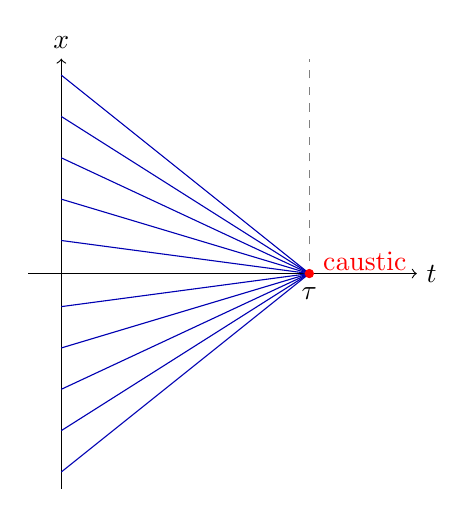
\begin{tikzpicture}[scale=1.05]
\draw[->] (-0.4,0) -- (4.3,0) node[right] {$t$};
\draw[->] (0,-2.6) -- (0,2.6) node[above] {$x$};
\draw[dashed,gray] (3,-0.05) -- (3,2.6);
\node[below] at (3,-0.05) {$\tau$};
\foreach \xa in {-2.4,-1.9,-1.4,-0.9,-0.4,0.4,0.9,1.4,1.9,2.4}{
  \draw[thin,blue!70!black] (0,\xa) -- (3,0);
}
\filldraw[red] (3,0) circle (1.4pt);
\node[right,red] at (3.05,0.15) {caustic};
\end{tikzpicture}
\caption{Characteristics $x(t;x_0)=x_0(1-t/\tau)$ of the free particle with
    converging initial phase $S_0(x)=-\frac{m}{2\tau}x^2$. Every trajectory,
    however far from the origin it starts, reaches $x=0$ at the same instant
    $t=\tau$: a caustic forms in finite time even though $V\equiv0$.}
\label{fig:focus}
\end{figure}

Take $V(x)=\tfrac12 m\omega^2x^2$, so $V''\equiv m\omega^2$ is constant, and
\eqref{hj:jacobi} becomes the harmonic-oscillator equation itself,
\[
\ddot J + \omega^2 J = 0, \qquad J(0,x_0)=1,\quad \dot J(0,x_0)=\frac{S_0''(x_0)}{m},
\]
with exact solution
\begin{equation}
J(t,x_0) = \cos\omega t + \frac{S_0''(x_0)}{m\omega}\sin\omega t.
\label{hj:Jsho}
\end{equation}

\begin{theorem}[Universal breakdown]
\label{thm:sho}
For the harmonic oscillator, for \emph{every} $S_0\in C^2(\mathbb{R})$ and
    \emph{every} $x_0\in\mathbb{R}$, the classical HJE solution starting from
    $x_0$ breaks down at the finite time
\begin{equation}
t^\ast(x_0) = \frac{1}{\omega}\left[\frac{\pi}{2} + \arctan\!
    \left(\frac{S_0''(x_0)}{m\omega}\right)\right] \ \in\ \Big(0,\ 
    \frac{\pi}{\omega}\Big).
\label{hj:tstarsho}
\end{equation}
In particular $t^\ast(x_0) < \pi/\omega$ uniformly in $x_0$ and in $S_0$: 
    no choice of smooth initial phase, however gentle, avoids a caustic within one half-period of the oscillator.
\end{theorem}

\begin{proof}
Write $A=1$, $B=S_0''(x_0)/(m\omega)$, so $J(t,x_0)=A\cos\omega t+B\sin\omega t
    = R\cos(\omega t-\phi)$ with $R=\sqrt{A^2+B^2}>0$ and
    $\phi=\arctan(B/A)=\arctan B\in(-\tfrac\pi2,\tfrac\pi2)$ (the branch is
    fixed by $A=1>0$). The zeros of $J$ are at $\omega t-\phi=\tfrac\pi2+k\pi$,
    $k\in\mathbb Z$, i.e. $t=(\phi+\tfrac\pi2+k\pi)/\omega$. Since
    $\phi\in(-\tfrac\pi2,\tfrac\pi2)$, the value at $k=0$ lies in
    $(0,\pi/\omega)$ and is manifestly the smallest positive root (the $k=-1$
    root is negative). This proves \eqref{hj:tstarsho}.
\end{proof}

Sanity checks on \eqref{hj:tstarsho}: if $S_0''(x_0)=0$ (locally ``flat''
data), $t^\ast=\pi/(2\omega)$, a quarter period. As $S_0''(x_0)\to+\infty$
(strongly diverging data), $t^\ast\to\pi/\omega$ but never reaches it. As
$S_0''(x_0)\to-\infty$ (strongly focusing data), $t^\ast\to0^+$: an
already-converging beam focuses almost instantly, exactly as one would guess.
What Theorem~\ref{thm:sho} adds is that \emph{even the most favorable, most
divergent possible data cannot postpone the caustic past $t=\pi/\omega$}. This
finite, data-independent interval between conjugate points is a classical fact
about the harmonic oscillator and is the
mechanical origin of the Maslov index increasing by one unit every half-period
in the semiclassical (Bohr--Sommerfeld--Maslov) quantization of the oscillator.

Theorem~\ref{thm:sho} is not special to the exactly quadratic potential; it is
the model case of a much more general comparison principle.

\begin{theorem}
\label{thm:sturm}
Suppose $V\in C^2(\mathbb{R})$ satisfies $V''(x)\ge m\omega^2$ for all
    $x\in\mathbb{R}$, for some $\omega>0$. Then for every $S_0\in
    C^2(\mathbb{R})$ and every $x_0\in\mathbb{R}$,
\[
t^\ast(x_0) < \frac{\pi}{\omega}.
\]
\end{theorem}

\begin{proof}
Along the trajectory, $q(t):=V''\big(x(t;x_0)\big)/m \ge \omega^2$ for all $t$,
    so $J$ solves $\ddot J + q(t)J=0$ with $J(0,x_0)=1\ne0$. Let
    $y(t)=\sin\omega t$, which solves $\ddot y+\omega^2y=0$ and has consecutive
    zeros at $t=0$ and $t=\pi/\omega$, with $y\ne0$ in between. By the Sturm
    comparison theorem applied to $\ddot J+qJ=0$ against $\ddot
    y+\omega^2y=0$ with $q\ge\omega^2$, $J$ must vanish somewhere in
    $(0,\pi/\omega)$ unless $J$ is a constant multiple of $y$ -- impossible
    here since $J(0,x_0)=1\ne 0=y(0)$.
\end{proof}

\begin{remark}
Theorem~\ref{thm:sturm} is the exact one-dimensional mechanical analogue of the
    Rauch comparison theorem in Riemannian geometry, in which $V''$ plays the 
    role of sectional curvature: a
    lower bound on curvature (here, on the ``restoring strength'' of the
    potential) forces conjugate points to appear within a bounded distance --
    the mechanical cousin of the Bonnet--Myers theorem. Convexity of $V$ is
    what does the damage; potentials that are flat or concave ($V''\le0$)
    behave more like the free particle of Section~\ref{sec:free}, where global
    existence is possible but only for a non-generic (convex) subset of initial
    data.
\end{remark}

It is tempting, on seeing \eqref{hj:jacobi} blow down to zero, to think of this
as a shock wave forming out of smooth data, as in Burgers' equation. The
analogy is real but must be handled carefully, because taken too literally it
suggests the wrong physical resolution.

Differentiating \eqref{hj:hjeq1} once in $x$ and writing $p=\partial_xS$ gives
the momentum-field equation
\begin{equation}
\partial_tp + \frac{1}{m}\,p\,\partial_xp = -V'(x).
\label{hj:burgers}
\end{equation}
For $V\equiv0$ this is exactly the inviscid Burgers equation for $u=p/m$, whose
characteristics are the same straight lines drawn in Figure~\ref{fig:focus}. So
far the analogy is exact. But there is a crucial difference in what the
crossing of characteristics \emph{means}.

Consider the full phase-space curve
\[
\Lambda_t := \big\{(x(t;x_0),p(t;x_0)) : x_0\in\mathbb{R}\big\} \subset \mathbb{R}^2.
\]
Because the Hamiltonian flow generated by \eqref{hj:ham} is, for the potentials
considered here, a complete flow of smooth diffeomorphisms of the phase plane
for all $t\in\mathbb{R}$, the curve $\Lambda_t$ is perfectly smooth for
\emph{every} $t$ -- nothing in phase space ever collides, merges, or loses
information: this is just Liouville's theorem together with uniqueness of
solutions of Hamilton's equations. What happens at $t=t^\ast(x_0)$ is entirely
a statement about the \emph{projection}
\[
\pi:\Lambda_t\to\mathbb{R}_x, \qquad (x,p)\mapsto x,
\]
whose derivative along $\Lambda_t$ at the point labelled by $x_0$ is exactly
$J(t,x_0)$. At $t=t^\ast(x_0)$, $\pi$ develops a critical point: $\Lambda_t$ is
momentarily tangent to the fibre direction there. This is a \emph{fold}, in the
sense of Whitney and Thom's theory of singularities of smooth maps (see Arnold
\cite{ArnoldCatastrophe} for an accessible account); immediately afterward,
$\pi$ is locally two-to-one, and two distinct sheets of $\Lambda_t$ -- two
distinct momenta -- sit over the same $x$. This is precisely a \emph{caustic}
in the sense of geometric optics: the bright curve on the floor of a swimming
pool, the cusp of a rainbow, the focal point of a lens in
Figure~\ref{fig:focus}. Rays (here, classical trajectories) do not disappear or
merge at a caustic; they simply cross, and go on to occupy the same point in
configuration space while carrying different momenta.

This is fundamentally different from a genuine shock in a scalar conservation
law, such as \eqref{hj:burgers} interpreted on its own as an evolution equation
for $p$ with, say, an entropy condition imposed to select a unique
discontinuous weak solution. That construction is appropriate for a dissipative
medium -- pressureless, sticky ``dust'' in which colliding particles merge and
information is genuinely lost, enforcing the Rankine--Hugoniot / Oleinik
entropy condition. It is not appropriate for the actual, collisionless
mechanical system \eqref{hj:hameqs} describes, in which trajectories pass
through one another. The two constructions coincide as pieces of formal
mathematics (the Lax--Oleinik entropy solution of \eqref{hj:burgers} is
literally $\partial_x$ of the Crandall--Lions viscosity solution of
\eqref{hj:hjeq1}, but they answer
different physical questions. This distinction is exactly the one drawn, in a
cosmological setting, between the ``adhesion approximation'' (dust that sticks
upon crossing, described by the entropy solution) and the true collisionless
dynamics of the Zel'dovich approximation to large-scale structure formation, in
which multiple streams of matter coexist after crossing and form a genuinely
multivalued velocity field.

Given that no single-valued classical solution survives past the first caustic,
there are two standard, and genuinely different, ways to say something about
$t>t^\ast$.

The honest object that continues smoothly through the caustic is not $S(x,t)$
but the Lagrangian curve $\Lambda_t$ itself, which remains smooth for all time.
Near a fold, $\Lambda_t$ is more naturally parametrized by $p$ (or by
arclength) than by $x$, and the correct statement of ``the solution'' becomes:
locally, finitely many smooth branches $S_1(x,t),S_2(x,t),\dots$, one for each
sheet of $\Lambda_t$ lying over $x$.

This is exactly what happens, one order more precisely, in the semiclassical
(WKB) approximation to the Schr\"odinger equation. Substituting
$\psi(x,t)\approx A(x,t)e^{iS(x,t)/\hbar}$ into the Schr\"odinger equation and
expanding in powers of $\hbar$ produces \eqref{hj:hjeq1} at leading order and a
transport equation for $A$ at the next order, with $A\propto |J|^{-1/2}$; the
WKB amplitude literally diverges at the caustic, exactly where $J=0$. The
correct continuation is a coherent sum over the branches, each carrying an
extra phase $-i\pi\mu_j/2$ where $\mu_j$ (the Maslov index of that branch)
counts the conjugate points crossed so far; near the caustic itself, this
asymptotic sum must be replaced by an Airy-function uniform approximation.

Alternatively, one can insist on a single-valued function of $(x,t)$ defined
for \emph{all} time, at the cost of giving up smoothness. Define
\begin{equation}
S(x,t) \ :=\ \inf\Big\{\, S_0\big(\gamma(0)\big) + \int_0^tL\big(\gamma(\tau),
    \dot\gamma(\tau)\big)\,d\tau \ :\ \gamma \text{ absolutely continuous},
    \ \gamma(t)=x \,\Big\},
\label{hj:hopflax}
\end{equation}
minimizing the total ``cost'' over \emph{all} paths ending at $x$ at time $t$,
with free initial point weighted by $S_0$. Because $L(x,\dot x)=\tfrac12m\dot
x^2-V(x)$ is strictly convex and superlinear in $\dot x$, this variational
problem is well posed for reasonable $V$ (e.g. bounded below, as for both
examples above), and \eqref{hj:hopflax} defines the unique \emph{viscosity
solution} of the Cauchy problem \eqref{hj:hjeq1}.

This $S$ agrees with the classical smooth solution of Theorem~\ref{thm:local}
for $t<t^\ast$, but for $t\ge t^\ast$ it typically develops a genuine kink -- a
jump in $\partial_xS$ -- exactly where two or more competing paths tie for the
minimum in \eqref{hj:hopflax}. In other words, \eqref{hj:hopflax} \emph{can} be
solved globally in time, but only by (i) discarding all but the single
\emph{minimal-action} branch at each point -- throwing away the very
trajectories whose mutual interference is physically encoded in the multivalued
WKB picture -- and (ii) accepting a solution that is merely Lipschitz, not
$C^1$, and therefore no longer ``the'' generating function of a canonical
transformation in the sense classical mechanics requires. This is the precise,
sharp form of the opening claim: a global solution in the classical
(single-sheeted, $C^1$) sense generically does not exist, and neither of the
two standard substitutes -- the multivalued semiclassical one or the
single-valued viscosity one -- is that classical solution; each recovers it
only for $t<t^\ast$ and replaces it with something structurally different
afterward.

The point of working out the free particle and the harmonic oscillator in such
elementary detail is to make it impossible to blame the phenomenon on some
contrived feature of $V(x)$. The free particle shows that the quadratic kinetic
term \emph{by itself} is enough to produce finite-time breakdown, for any
initial phase with a single region of concavity. The harmonic oscillator shows
that once any amount of convexity is added to $V$, breakdown becomes not merely
generic but \emph{unconditional}: literally no choice of $C^2$ initial data
survives past $t=\pi/\omega$. Between these two examples lies essentially every
problem discussed in an introductory mechanics course.

